%================================================================
\begin{frame}{Multilingual Semantic Representations}
%================================================================
\framesubtitle{Contact: Marianna Apidianaki (LIMSI) \& Olivier Ferret (CEA)}
Tasks~2 (Heterogeneous data and knowledge) and~3 (Machine learning)
\vfill

  \begin{columns}
    \begin{column}{5cm}
      \begin{center}
        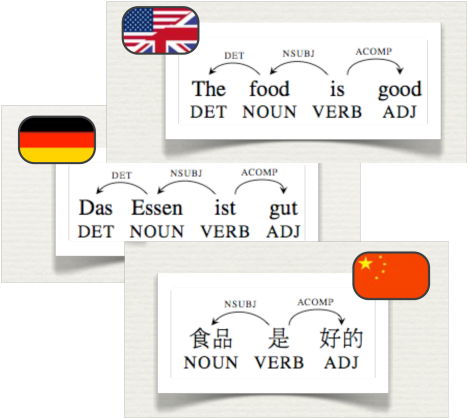
\includegraphics[width=\linewidth]{Images/rsm-multilingual-parsing.png}\\
        Universal Syntactic Processing (Petrov et al.)
      \end{center}
    \end{column}
    \begin{column}{5cm}
      Can one build representations which apply across languages?
    \end{column}
  \end{columns}

  \contacturl{http://labex-digicosme.fr/GT+Representations+Semantiques+Multilingues}
\end{frame}

%================================================================
\begin{frame}{Multilingual Semantic Representations}
  \framesubtitle{Activities: 8 teams in 6 laboratories, 66 registered researchers, 15--40 participants per meeting}

  \begin{center}
    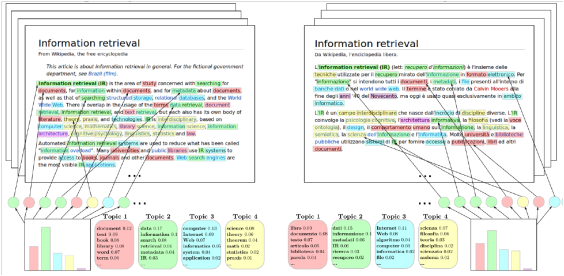
\includegraphics[width=0.65\linewidth]{Images/rsm-multilingual-space-bilda.png}\\
    Use of BiLDA (Vulic et al.)
  \end{center}
  \begin{columns}\small
    \begin{column}{5cm}
      Seminars:\\
      Slav Petrov (Google NYC, USA)\\
      Stephan Gouws (Deep WG; Stellenbosch U., South Africa)\\
      Fabian Suchanek (LTCI, Paris-Saclay)
    \end{column}
    \begin{column}{6cm}
      Ivan Vulic (KULeuven, Belgium)\\
      Roberto Navigli (Sapienza U.\ of Rome, Italy)\\
      Marine Carpuat (U.\ Maryland, USA)
    \end{column}
  \end{columns}

  \contacturl{http://labex-digicosme.fr/GT+Representations+Semantiques+Multilingues}
\end{frame}

%================================================================
\begin{frame}{Multilingual Semantic Representations}
  \framesubtitle{Activities}
  \begin{itemize}
  \item Six seminars + three work meetings
  \item Co-supervised Master internship (LIMSI-CEA, distributional analysis and terminology extraction)
    (and co-supervised PhD submission)
  \item Support for DigiCosme Invited Professor: see below, D2K
  \end{itemize}

  Outcomes:
  \begin{itemize}
  \item Led to ANR-DFG project GoASQ (ANR-DFG: LRI-LIMSI-TUD, 2016--2019) and ANR submission ADDICTE (\ldots-CEA-LIMSI)
  \item Led to WG Data to Knowledge (D2K)
\end{itemize}

\contacturl{http://labex-digicosme.fr/GT+Representations+Semantiques+Multilingues}
\end{frame}

%================================================================
\begin{frame}{Multilingual Semantic Representations}
\framesubtitle{Perspectives}
\begin{itemize}
\item More seminars, meetings, co-supervised internships
\item Links with Deep WG (mutually relevant seminars, e.g. S.~Gouws, E.~Grefenstette, A.~Bordes)
\item Continued links with D2K WG (see below, input to B2SRI Strategic Research Institute)
\end{itemize}

\contacturl{http://labex-digicosme.fr/GT+Representations+Semantiques+Multilingues}
\end{frame}

%================================================================
\begin{frame}{From Data to Knowledge}
%================================================================
\framesubtitle{Contact: Claire Nédellec, INRA ; Chantal Reynaud, LRI }
Task~2 (Heterogeneous data and knowledge), Task~3 (Machine learning), Task~1  (Large-scale data)
\begin{itemize}
\item Answering complex questions in scientific and technical domains
\item Combination of interdisciplinary methods
  \begin{itemize}
  \item to analyze, integrate, understand, predict data, information, knowledge
  \item heterogeneous, uncertain, contradictory, multi-scale, integrated, formalized
  \end{itemize}
\item Complexity of the \{data -- information -- knowledge\} iteration
  \begin{itemize}
  \item Information extraction and interpretation (text, image, exper.\ data\ldots)
  \item Formal languages for representation and usage
  \item User in the loop
  \end{itemize}
\end{itemize}

% HERE AN IMAGE ABOUT THE TOPIC OF THIS WG

\contacturl{http://labex-digicosme.fr/GT+D2K }
\end{frame}

%================================================================
\begin{frame}{From Data to Knowledge}
\framesubtitle{Activities: 12 laboratories involved, 18 teams, 64 registered researchers, about 20 participants per meeting}

Meetings topics (including 2 national and 1 international speakers):
\begin{itemize}
\item Information extraction from texts, ontologies
\item Modeling and processes
\item Knowledge and image analysis
\item Knowledge and reasoning
\item Multimedia content analysis
\end{itemize}

\contacturl{http://labex-digicosme.fr/GT+D2K }
\end{frame}

%================================================================
\begin{frame}{From Data to Knowledge}
\framesubtitle{Activities: Strategic reflexion}

Subgroup on \emph{Interface between Computer Science and Life Sciences, from Data to Knowledge}
  \begin{itemize}
  \item How can D2K topics contribute to shared projects with the Life Sciences Department of U.~Paris-Saclay?
  \item[$\rightarrow$] The topic \emph{CS for modeling living organisms} was registered as a priority topics in the Life Sciences Department SGT5
  \item[$\rightarrow$] Issued a document included in the appendix of the \emph{Life Sciences Department White Paper}
\end{itemize}

\contacturl{http://labex-digicosme.fr/GT+D2K }
\end{frame}

%================================================================
\begin{frame}{From Data to Knowledge}
\framesubtitle{Outcomes}

\begin{itemize}
\item Led to ANR-DFG project GoASQ (ANR-DFG: LRI-LIMSI-TUD, 2015--2019): \emph{Generating and Answering Ontological Queries over Semi-structured Data}
\item Contribution to the B2SRI Strategic Research Institute application
  \begin{itemize}
  \item Systems Biology and Synthetic Biology for Research and Innovation (Life Sciences + CS)
  \end{itemize}
\item Two teams collaborate in H2020 E-Infra OpenMinTeD: Open Mining Infrastructure for Text and Data (2015--2018)
\item DigiCosme Invited Professor: Kevin B.\ Cohen (U.\ Colorado), text mining in biomedicine (3 months, 2016)
\end{itemize}

\contacturl{http://labex-digicosme.fr/GT+D2K }
\end{frame}

% %================================================================
% \begin{frame}{From Data to Knowledge}
%   \framesubtitle{Perspectives}
%   \begin{itemize}
%   \item More seminars and meetings
%   \item More contribution to B2SRI Strategic Research Institute\\ depending on outcome of selection
%   \end{itemize}

%   \contacturl{http://labex-digicosme.fr/GT+D2K }
% \end{frame}

%================================================================
\begin{frame}{Building a cartographic map of scientific communities (SciCoSense) }
%================================================================
  \framesubtitle{Contact: Philippe Caillou, LRI}

  \begin{columns}
    \begin{column}{3cm}
      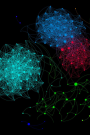
\includegraphics[width=\linewidth]{Images/scicosence-image.png}
    \end{column}
    \begin{column}{8cm}
      Task~2 (Heterogeneous data and knowledge), Task~1 (Large-scale data),
      Task~3 (Machine learning), Task~4 (interactive optimization),
      Task~5 (Visualization).\\
      Links to Lidexes `Center for Data Science' (CDS) and `Digital Society Institute' (ISN)
    \end{column}
  \end{columns}

  \contacturl{http://labex-digicosme.fr/GT+SciCoSense}
\end{frame}

%================================================================
\begin{frame}{Building a cartographic map of scientific communities (SciCoSense) }
  \framesubtitle{Topic and activities}
  Representation and study of social networks:
  \begin{itemize}
  \item Study scientific communities
  \item based on traces of their activities
  \item to build indicators, maps and query tools
  \item about scientific production
  \end{itemize}

  Joint meeting with Center for Data Science on the analysis of scientific papers.

  \contacturl{http://labex-digicosme.fr/GT+SciCoSense}
\end{frame}

%================================================================
\begin{frame}{Deep Learning and Distributed Representations}
%================================================================
\framesubtitle{Contact: Alexandre Allauzen, LIMSI ; Emmanuelle Frenoux, LIMSI }

  \begin{columns}
    \begin{column}{3cm}
      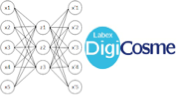
\includegraphics[width=\linewidth]{Images/deepnet1.png}
    \end{column}
    \begin{column}{8cm}
      DataSense Task~3 (Machine learning)\\[2ex]

      \emph{Topic:}\\
      Deep neural networks and representation learning\\[2ex]

      \emph{Activities:}
      \begin{itemize}
      \item Journal club
      \item Cross-team presentations
      \item Invited seminars
      \end{itemize}
    \end{column}

  \end{columns}
  \vfill

  \emph{Participants:}\\
    LIMSI, CNRS (TLP, AMI) ---
    LRI, CNRS \& UPSud (TAO) ---
    U2IS, ENSTA ---
    LTCI, Télécom-ParisTech


\contacturl{http://labex-digicosme.fr/GT+Reseaux+profonds }
\end{frame}

%================================================================
\begin{frame}{Deep Learning and Distributed Representations}
\framesubtitle{Activities (examples)}

14 meetings, among which some invited seminars:
\begin{itemize}
\item S.\ Lauly (U. Sherbrooke, Canada)
\item S.\ Gouws (U. Stellenbosch, South Africa)
\item A.\ Bordes (Facebook, New York / Paris)
\item E.\ Grefenstette (Google-Deepmind)
\item S.\ Mallat (ENS)
\item T.\ Cohen (Amsterdam University)
\item M.\ Riedmiller (Google-Deepmind) (soon)
\end{itemize}
\bigskip

Co-supervised Master internship then PhD

\contacturl{http://labex-digicosme.fr/GT+Reseaux+profonds }
\end{frame}


%================================================================
\begin{frame}{Apprentissage, décision séquentielle et robotique }
%================================================================
\framesubtitle{Contact: David Filliat, U2IS - ENSTA ParisTech}

\begin{minipage}[c]{.4\linewidth}
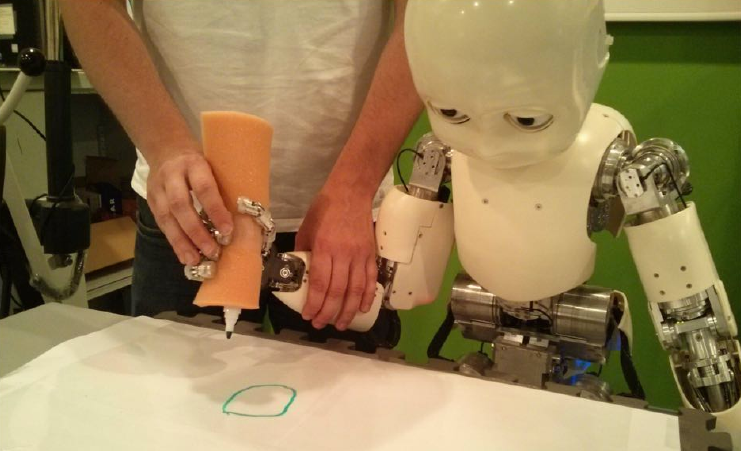
\includegraphics[width=\linewidth]{Images/robotique1.png}
\end{minipage} 
\hfill
\begin{minipage}[c]{.55\linewidth}
Objectives:
\begin{itemize}
\item Launch common actions on learning and robotics
\item Bring practical and  theoretical developments  in robotics
\item Funding of foreign speakers and master students
\end{itemize}
Members: U2IS,	LRI,	LIMSI,	ONERA,	UVSQ,	CEA	
\end{minipage} 
\contacturl{http://labex-digicosme.fr/GT+Robotique}
\end{frame}

%================================================================
\begin{frame}{Apprentissage, décision séquentielle et robotique }
\framesubtitle{Contact: David Filliat, U2IS - ENSTA ParisTech}


\begin{minipage}[c]{.4\linewidth}
      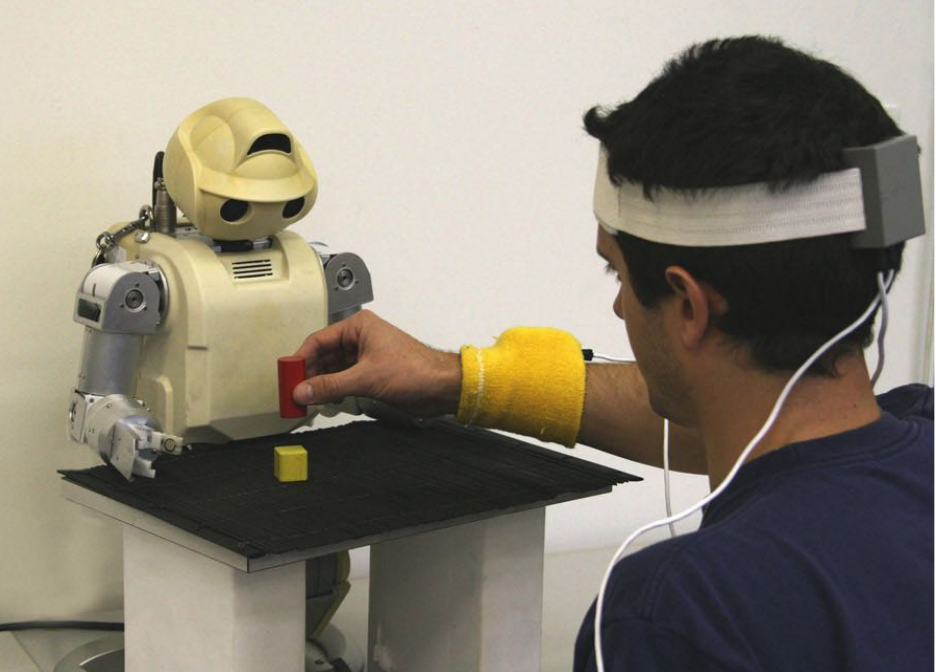
\includegraphics[width=\linewidth]{Images/robotique2.png}
   \end{minipage} \hfill
   \begin{minipage}[c]{.55\linewidth}
\textbf{Reinforcement learning} learning from preferences between examples provided by human interactions. Global cost function? Reduce the requirement on the number of training samples? \\
\textbf{Big data} better use learning data provided by robots, possibly with deep learning. Identification of useful visual features for a given task
   \end{minipage}
\begin{center}
6 invited talks.\\
one intern, one PhD thesis
\end{center}

\contacturl{http://labex-digicosme.fr/GT+Robotique}
\end{frame}

%================================================================
\begin{frame}{Prédiction et Analyse de données structurées et hétérogènes (PASADENA) }
%================================================================
\framesubtitle{Contact: Arthur Tenenhaus, Centrale-Supélec ; Florence d’Alché-Buc, Slim Essid,  Maxime Sangnier, Télécom-ParisTech}
\contacturl{http://labex-digicosme.fr/GT+PASADENA}

\begin{alertblock}{Objectives}
Developpement of statistical methods for complex data analysis: \textbf{heterogeneous}, \textbf{multimodal} and \textbf{structured} data:
\begin{itemize}
\item unsupervised analysis of correlations between modalities;
\item classification/regression from heterogeneous data;
\item structured prediction to fit a certain type of data from another;
\end{itemize}
\end{alertblock}


\begin{minipage}[c]{.7\linewidth}
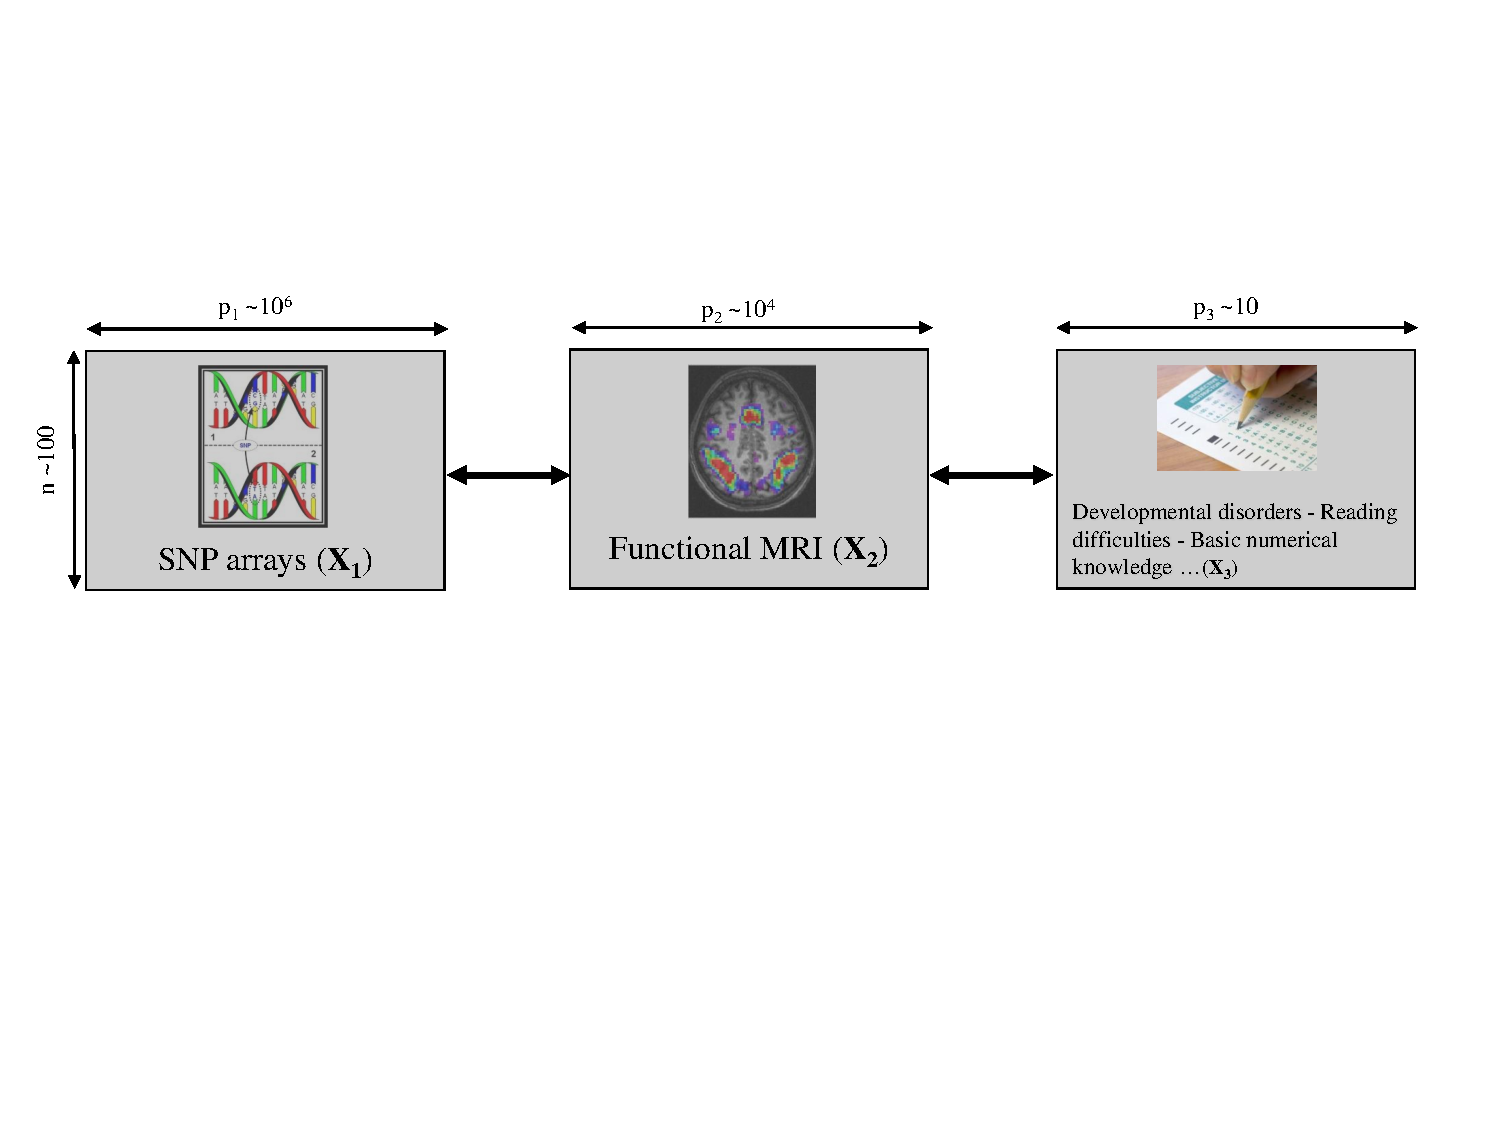
\includegraphics[trim = 0mm 90mm 0mm 50mm, clip, width=\linewidth]{Images/pasadena_poster_I.pdf}
\end{minipage}\hfill
\begin{minipage}[c]{.28\linewidth}
Multibloc study in imaging genetics.
\end{minipage}


\end{frame}


%================================================================
\begin{frame}{Prédiction et Analyse de données structurées et hétérogènes (PASADENA) }

\textbf{Example 2.} Supervised analysis can benefit from exploiting the structure in the data for the sake of computational efficiency

\begin{figure}
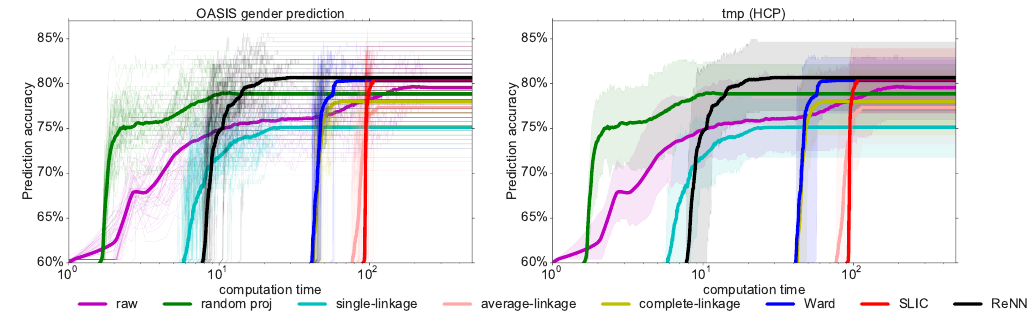
\includegraphics[trim = 0mm 0mm 0mm 0mm, clip = TRUE, width=1\linewidth]{Images/computation_time.png}
\caption{Massive data analysis: leveraging the data structure to achieve high computational gains \textbf{and} high prediction accuracy}
\label{comp_time}
\end{figure}
\end{frame}

%================================================================
\begin{frame}{Prédiction et Analyse de données structurées et hétérogènes (PASADENA) }

\textbf{Example 3.} Unsupervised grouping of speakers by co-factorization of non-negative matrices on audio/video data.

\vspace{1cm}
\begin{figure}
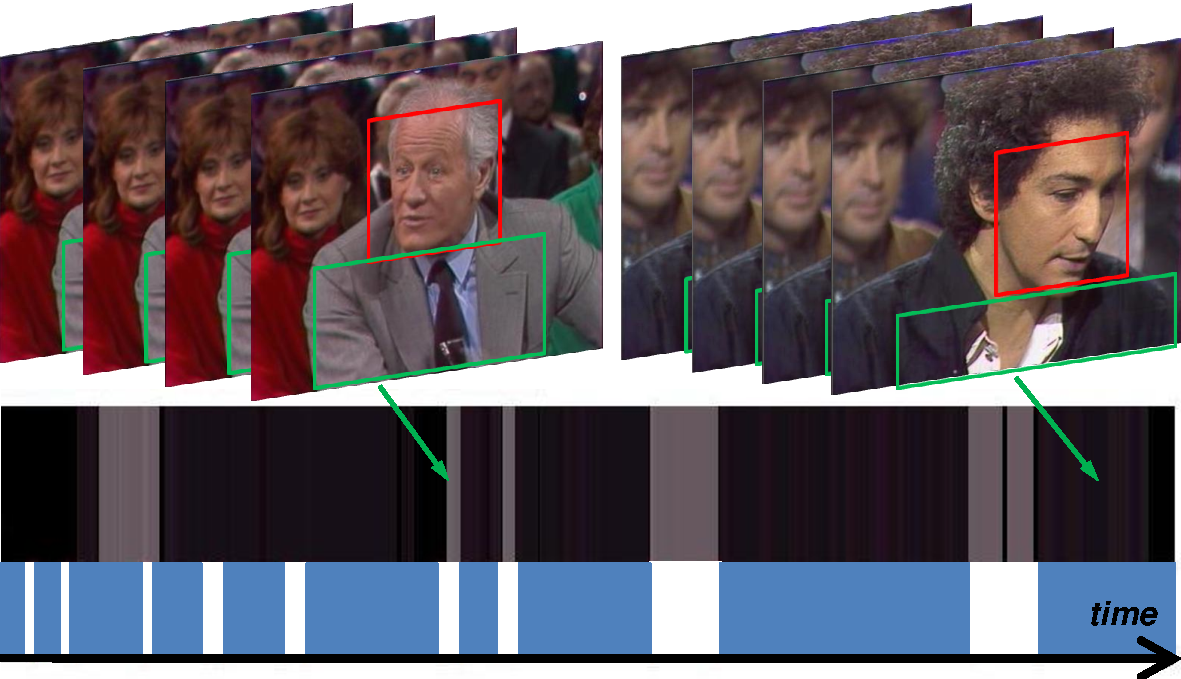
\includegraphics[trim = 0mm 0mm 0mm 0mm, clip = TRUE, width=.75\linewidth]{Images/2_speaker_turns.pdf}
\caption{Temporal segmentation by NMF.}
\end{figure}

\end{frame}

%================================================================
\begin{frame}{Machine Learning with scikit learn}
%================================================================
\framesubtitle{Contact: Olivier Grisel, Inria Saclay}

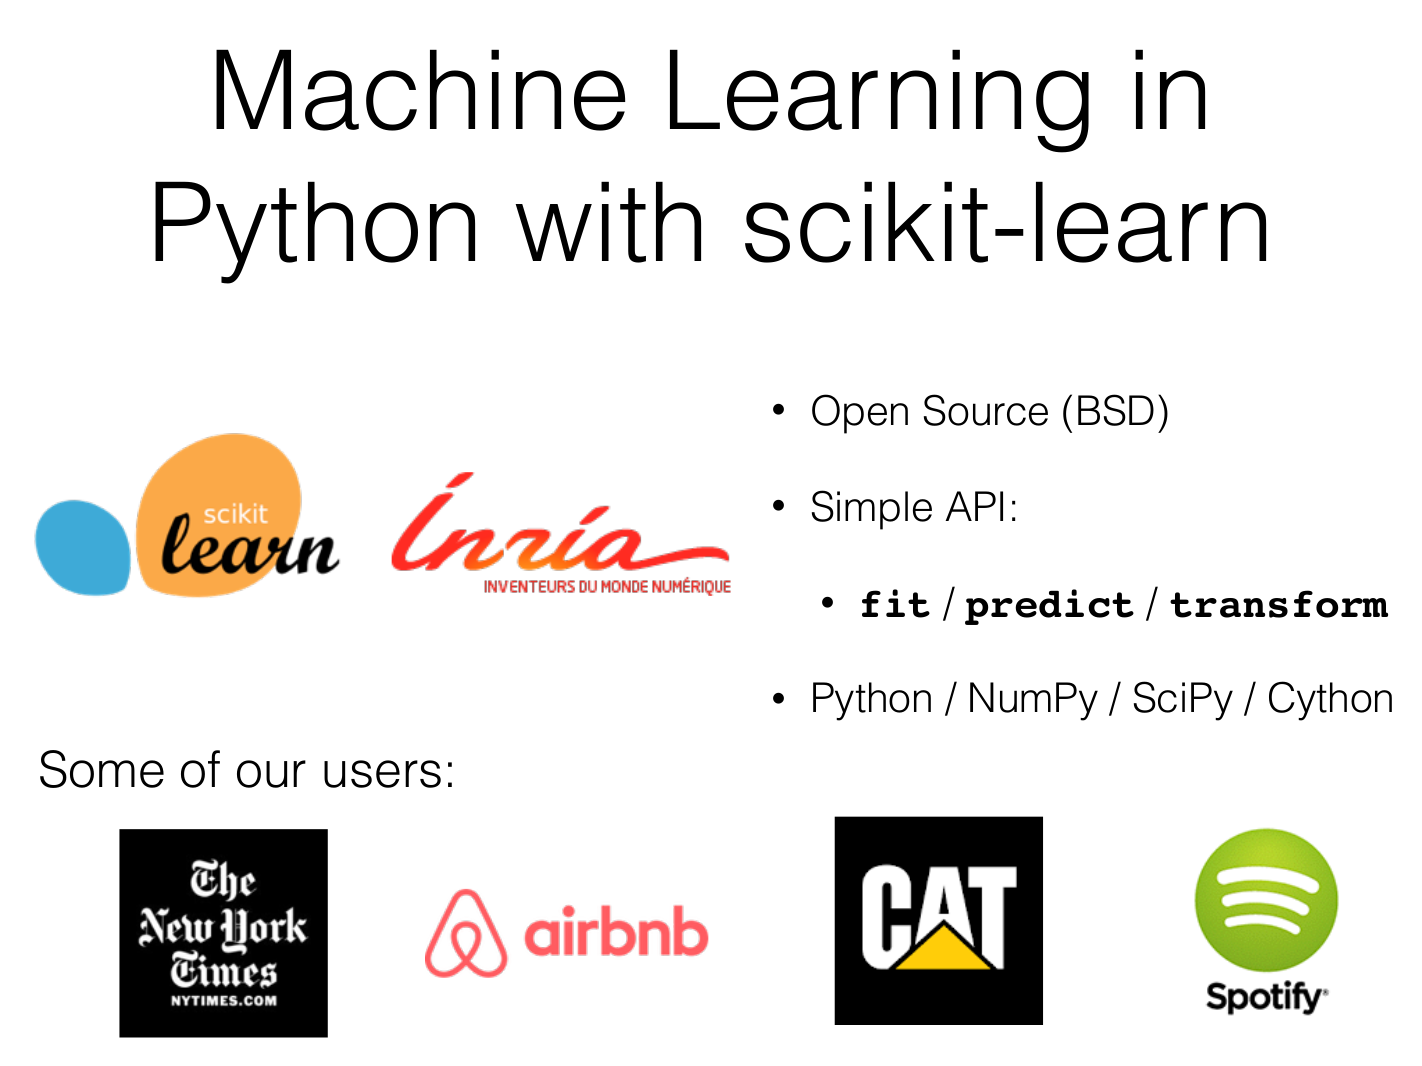
\includegraphics[trim = 0mm 0mm 0mm 0mm, clip = TRUE, width=.7\linewidth]{Images/skl.png}

\contacturl{http://scikit-learn.org}
\end{frame}

%================================================================
\begin{frame}{Human-Robot Interaction}
%================================================================
\framesubtitle{Contact: Laurence Devillers \& Jean-Calude Martin (LIMSI-CNRS) }

\begin{minipage}[c]{.4\linewidth}
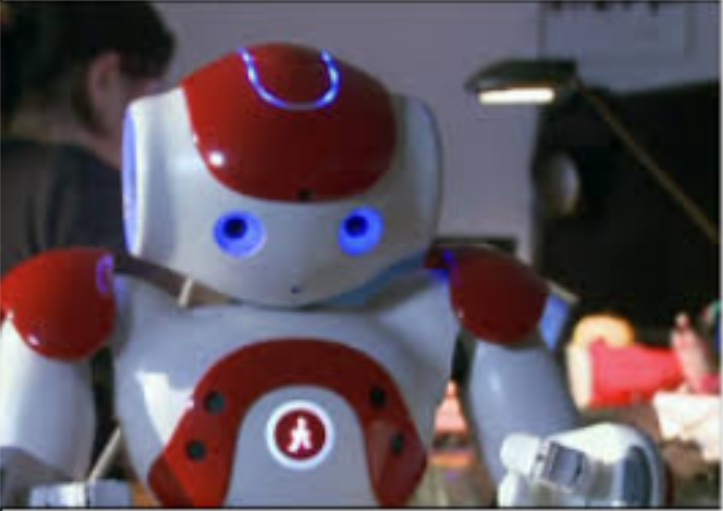
\includegraphics[width=\linewidth]{Images/hr1.png}
\end{minipage} 
\hfill
\begin{minipage}[c]{.55\linewidth}
Objectives
\begin{itemize} 
\item Create a community on interactive robotics; verbal/non-verbal/physical Human-robot interactions 
\item Group specialists beyond robotics: modeling and interaction, big data, psychology, social and cognitive sciences, ergonomy and  usage, ethics.
\end{itemize}
 Members : LIMSI, ENSTA, CEA, Télécom SudParis, Télécom ParisTech, Télécom Ecole de Management, Université Paris-Sud, UVSQ, Université d’Evry, CERDI
\end{minipage}

\contacturl{http://labex-digicosme.fr/GT+Interaction }
\end{frame}

%================================================================
\begin{frame}{Human-Robot Interaction}
\framesubtitle{Contact: Laurence Devillers \& Jean-Calude Martin (LIMSI-CNRS) }

\begin{minipage}[c]{.3\linewidth}
Main themes\\

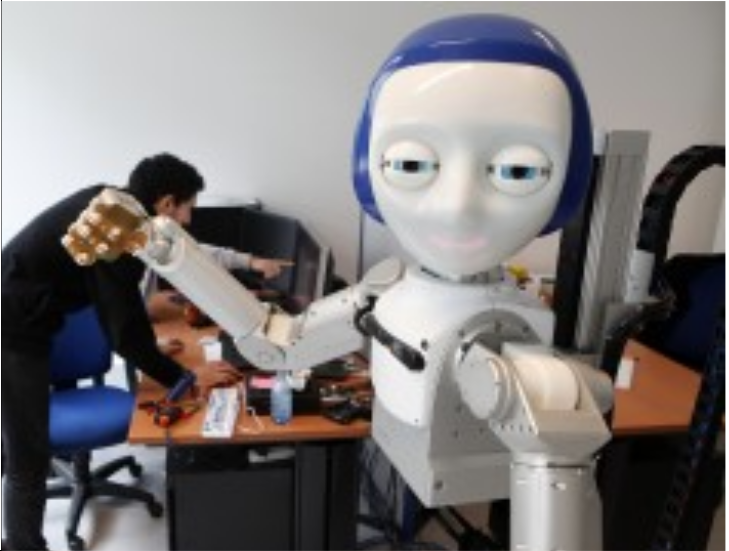
\includegraphics[width=\linewidth]{Images/hr2.png}
\end{minipage} 
\hfill
\begin{minipage}[c]{.67\linewidth}
\begin{itemize}
\item Affective and social dimensions of spoken interactions, H/R dialog, virtual agents/emotion, virtual reality  (LIMSI-CNRS)
\item Robotics and vision (ENSTA) Audio, Acoustics and waves -  Multimedia (LTCI-Télécom ParisTech)
\item Interactive Robotics (LISV-UVSQ) Assistance and interaction (LISV-UVSQ) Robotics and health – Interactive robotics (CEA-LIST)
Intermedia (Télécom SudParis) HANDS - HANDicap et health (IBISC-Univ. Evry)
\item Sociology, Psychology et Ergonomy (Télécom ParisTech –(I3)) UCOTIC teamlaw and robots - CERDI
\end{itemize}
\end{minipage} 

\contacturl{http://labex-digicosme.fr/GT+Interaction }
\end{frame}

%================================================================
\begin{frame}{Human-Robot Interaction}
  \framesubtitle{Announcement}

  Shared conference:
  \begin{itemize}
  \item Interactive Robotics at Paris-Saclay
  \item E3-ROBOTIC: Experimentation/Evaluation/Ethics and usages in InteraCtive ROBOTics
  \item Research, demos, collaborations, challenges, projects, industries in interactive robotics
  \item Date: 20 May 2016 --- Location: ENSTA
  \end{itemize}

  \contacturl{http://labex-digicosme.fr/GT+Interaction }
\end{frame}



%%% Local Variables: 
%%% mode: latex
%%% coding: utf-8-unix
%%% ispell-local-dictionary: "english"
%%% TeX-master: "datasense-2016.tex"
%%% fill-column: 9999
%%% End: 
